\documentclass[12pt]{article}

\usepackage{Preamble}

%! Author = sbbfti
%! Date = 10/06/2020

\newacronym{ADF}{ADF test}{Augmented Dickey-Fuller test}
\newacronym{KPSS}{KPSS test}{Kwiatkowski-Phillips-Schmidt-Shin test}
\newacronym{ACF}{ACF}{AutoCorrelation function}
\newacronym{PACF}{PACF}{Partial AutoCorrelation function}


\newacronym{ti}{$T_{i}$}{indoor air temperature, $^{\circ}$C}


\title{Assignment \#4}				% Title
\author{Saeed Kazemi}				% Author
\date{\today}						% Date

\makeatletter
\let\theauthor\@author
\let\thedate\@date
\let\thetitle\@title
\makeatother
\begin{document}

%%%%%%%%%%%%%%%%%%%%%%%%%%%%%%%%%%%%%%%%%%%%%%%%%%%%%%%%%%%%%%%%%


\begin{titlepage}
	\centering
    \vspace*{0.4 cm}
    
\includegraphics[scale = 0.5]{figures/unb.jpg}\\[1.0 cm]	% University Logo
    \textsc{\LARGE \newline\newline University of New Brunswick}\\[1.8 cm]	% University Name
	\textsc{\Large Time Series Analysis\\(EE 6563)}\\[0.5 cm]				% Course Code
	\rule{\linewidth}{0.2 mm} \\[0.4 cm]
	{ \huge \bfseries \thetitle}\\
	\rule{\linewidth}{0.2 mm} \\[1.5 cm]
	
	\begin{minipage}{0.5\textwidth}
		\begin{flushleft} \large
			\emph{Professor:}\\
			Erik Scheme\\
            Electrical and Computer Engineering\\
			\end{flushleft}
			\end{minipage}~
			\begin{minipage}{0.5\textwidth}
            
			\begin{flushright} \large
			\emph{Author:} \\
			Saeed Kazemi\\ (3713280)\\

		\end{flushright}
        
	\end{minipage}\\[1 cm]
	
	
    \thedate
    
    
    
	
\end{titlepage}

%%%%%%%%%%%%%%%%%%%%%%%%%%%%%%%%%%%%%%%%%%%%%%%%%%%%%%%%%%%%%%%%%



%\tableofcontents
\pagebreak

%%%%%%%%%%%%%%%%%%%%%%%%%%%%%%%%%%%%%%%%%%%%%%%%%%%%%%%%%%%%%%%%%
%================================================================
\begin{enumerate}

\item \textbf{Explore the attached dataset and find additional information from the resources listed below.  Note that this is the same dataset as was used in assignment 2.}
\begin{enumerate}
\item The dataset comprises NY Stock Exchange with several additional predictors, as explained in the following paper (especially sections 5 and 6):  (\href{https://www.sciencedirect.com/science/article/abs/pii/S0957417419301915}{ Source}).
\item The original dataset was obtained from: (\href{https://archive.ics.uci.edu/ml/datasets/CNNpred\%3A+CNN-based+stock+market+prediction+using+a+diverse+set+of+variablesc}{ This link}).
\item Although the original dataset includes 5 different files, we will only use the "NYSE.csv" file, which includes values from 2010 to 2017.
\end{enumerate}



%%%%%%%%%%%%%%%%%%%%%%%%%%%%%%%%%%%%%%%%%%%%%%%%%%%%%%%%%%%%%%%%%
%%%%%%%%%%%%%%%%%%%%%%%% Question 1 %%%%%%%%%%%%%%%%%%%%%%%%%%%%%
%%%%%%%%%%%%%%%%%%%%%%%%%%%%%%%%%%%%%%%%%%%%%%%%%%%%%%%%%%%%%%%%%
\newpage
\item \textbf{Hold out the last 3 months of 2017 for out-of-sample prediction and implement the following:} 
\begin{enumerate}
\item \textbf{Begin by forecasting with a single LSTM-layer and optimize its performance by varying the various hyper-parameters, for example: LSTM units, no. of layers, batch  size, learning  rate, etc. Plot and analyze the model performance (accuracy and loss) vs. the number of epochs. You should also test different  techniques to avoid model overfitting. Be sure to include and  contrast examples of the different approaches – don’t only show “the best”. Plot the predictions and report the forecasting error using appropriate metrics.}
\item \textbf{Repeat the forecasting using a 1D CNN-based  forecasting model. Evaluate and optimize its performance similar to point part (a). This may require you to go beyond course material, but there are plenty of resources online that you can leverage.}
\item \textbf{Now, implement a hybrid ConvLSTM forecasting model by combining the CNNs and LSTMs together. Evaluate and optimize its performance in comparison to part (a) and (b). Plot the predictions and report the forecasting error using appropriate metrics in comparison to part (a) and (b).}
\end{enumerate}

\textit{Figure \ref{fig:ass4_frameworks} depicts my framework for all three parts of this assignment. For each part we used the same procedure but with different architectures for DNN. In the following I discuss about each step.  }

\begin{figure}[H]
    \centering
    \begin{minipage}[b]{1.1\textwidth}
        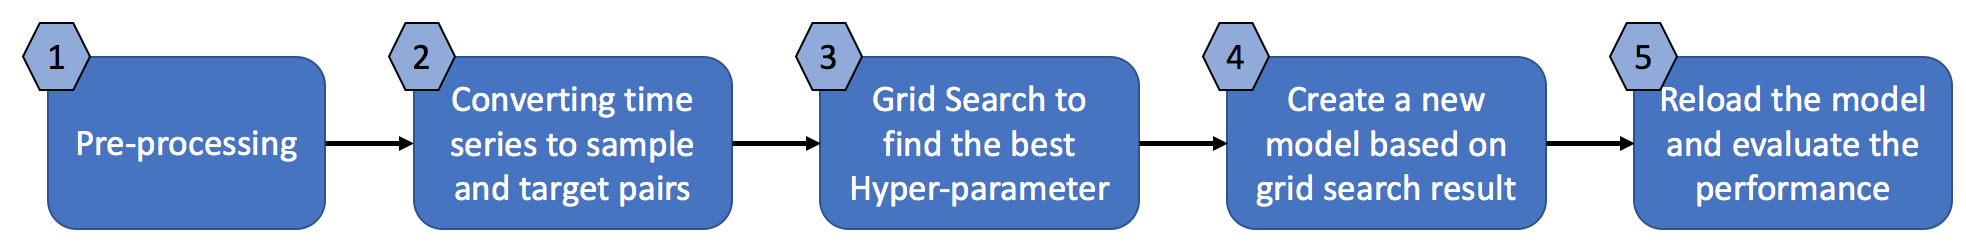
\includegraphics[width=\textwidth]{manuscript/src/figures/Ass4/Ass4_frameworks.png}
    \end{minipage}
    \caption{The framework that was used for this question.}
    \label{fig:ass4_frameworks}
\end{figure}


\textit{In pre-processing step, we used the last 570 samples for test and others for training set. This part is equal to the last three years. Then the MinMax function was used to change the input scaling between zero and one due to the fact that signal range was large. for this purpose, I used training set for finding min and max value, and then transformed both training and test set based on these two values. }


\textit{In the next step, I have converted normalized time-series data to pairs samples and output, or in other words, the supervised data. For doing this, I have used create\_dataset() function from the tutorial code. This function needs two arguments time-series signal and window size and returns a sequence of signal based on window size as input, and then the next value considered as output. The below image depicts this converting with the window size of 3. For this question, the window size set to 15.}

\begin{figure}[H]
     \centering
     \begin{subfigure}[b]{0.55\textwidth}
         \centering
         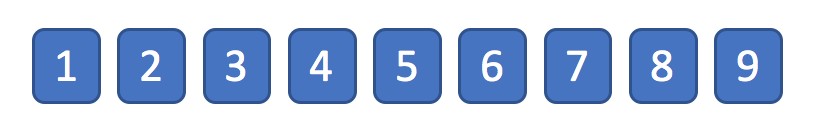
\includegraphics[width=1\textwidth]{manuscript/src/figures/Ass4/time.png}
         \caption{The time-series signal.}
         \label{fig:ROC_all}
     \end{subfigure}
     \vfill
     \begin{subfigure}[b]{.25\textwidth}
         \centering
         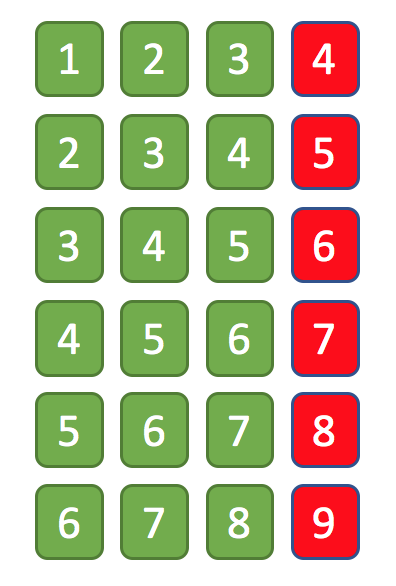
\includegraphics[width=1\textwidth]{manuscript/src/figures/Ass4/sup.png}
         \caption{Samples sequence with corresponding output values.}
         \label{fig:ROC_fcn}
     \end{subfigure} 
        \caption{Converting time-series signal to the supervised data. For this example, window size is equal to 3. }
        \label{fig:ROC}
\end{figure}

\textit{To optimize our model, I have used grid search to find the best hyper-parameters. Since grid search is a function on the Scikit-learn libraty, we needed to convert Keras model to a Scikit-learn model. So that I imported KerasClassifier from "keras.wrappers.scikit\_learn". Then a GridSearchCV instance was made based on our model, the search space, and 5-fold cross-validation object. Tables \ref{tab:Ass4_Q2a} to \ref{tab:Ass4_Q2c} show the search space of grid search as well as the best hyper-parameters for our model for all three parts of this question. }


\begin{table}[H]
\centering
\caption{The search space of GridSearchCV method as well as the best hyper-parameters for part (a).}
\label{tab:Ass4_Q2a}
\begin{lstlisting}
param_grid=
    {
        'LSTM_units':       [5, 15, 10],
        'batch_size':       [16, 32, 64],
        'learning_rate':    [0.0001, 0.001, 0.01]
    }

Best hyper-parameters=
    {
        'LSTM_units':       10,
        'batch_size':       16, 
        'learning_rate':    0.01
     }
\end{lstlisting}



\end{table}

\begin{table}[H]
\centering
\caption{The search space of GridSearchCV method as well as the best hyper-parameters for part (b).}
\label{tab:Ass4_Q2b}
\begin{lstlisting}
param_grid=
    {
        'batch_size':       [16, 32, 64],
        'learning_rate':    [0.0001, 0.001, 0.01]
    }

Best hyper-parameters=
    {
        'batch_size':       16, 
        'learning_rate':    0.01
     }
\end{lstlisting}
\end{table}


\begin{table}[H]
\centering
\caption{The search space of GridSearchCV method as well as the best hyper-parameters for part (c).}
\label{tab:Ass4_Q2c}
\begin{lstlisting}
param_grid=
    {
        'batch_size':       [16, 32, 64],
        'learning_rate':    [0.0001, 0.001, 0.01]
    }

Best hyper-parameters=
    {
        'batch_size':       64, 
        'learning_rate':    0.01
     }
\end{lstlisting}

\end{table}

 

\textit{After optimizing hyper-parameters, a new model have been created according to the best hyper-parameters of last step. Then the model was trained with 100 epochs. Also validation split was set to 0.2 that means 20 percent of the training data to be used as validation data. Validation data was used for avoiding the overfitting problem. Moreover, a callback method was used to track the loss function on training and validation set. The callback called only in training phase with model.fit() function to save a best model in a checkpoint file, so the model could be loaded later. Tables \ref{Ass4_Q2a_result} to  \ref{Ass4_Q2c_result} indicate the results of overtrained and trained models on the test and train set. }

\begin{table}[H]
\centering
\caption{The results of overtrained and trained models on the test and train set for part (a).}
\label{tab:Ass4_Q2a_result}
\begin{tabular}{lr}
\toprule
{} & {}
\midrule
RMSE of overtrained model on Train set: & 104.90 \\
RMSE of trained model on Train set: & 101.44 \\
RMSE of overtrained model on Test set: & 113.96 \\
RMSE of trained model on Test set:  & 111.85 \\

\bottomrule
\end{tabular}
\end{table}

\begin{table}[H]
\centering
\caption{The results of overtrained and trained models on the test and train set for part (b).}
\label{tab:Ass4_Q2b_result}
\begin{tabular}{lr}
\toprule
{} & {}
\midrule
RMSE of overtrained model on Train set: & 128.27 \\
RMSE of trained model on Train set: & 134.87 \\
RMSE of overtrained model on Test set: & 313.35 \\
RMSE of trained model on Test set:  & 186.67 \\

\bottomrule
\end{tabular}
\end{table}


\begin{table}[H]
\centering
\caption{The results of overtrained and trained models on the test and train set for part (c).}
\label{tab:Ass4_Q2c_result}
\begin{tabular}{lr}
\toprule
{} & {}
\midrule
RMSE of overtrained model on Train set: & 488.72 \\
RMSE of trained model on Train set: & 164.46 \\
RMSE of overtrained model on Test set: & 929.16 \\
RMSE of trained model on Test set:  & 356.09 \\

\bottomrule
\end{tabular}
\end{table}





\textit{For part b, Fully Convolutional Networks (FCN) \cite{WangTimeBaseline} has been implemented. This model is a end-to-end convolutional network with three blocks. Each block has a convolutional layer followed by a batch normalization and ReLU activation layer. The output of the third block is averaged over the time dimension which corresponds to global average pooling (GAP) layer. Finally, a dense layer is fully connected to the GAP layer’s output to produce the final prediction.}

\textit{For part c, the FCN used in a sequential order. Furthermore, all models used Adam algorithm as their optimization.}




























\begin{figure}[H]
    \centering
    \begin{minipage}[b]{1\textwidth}
        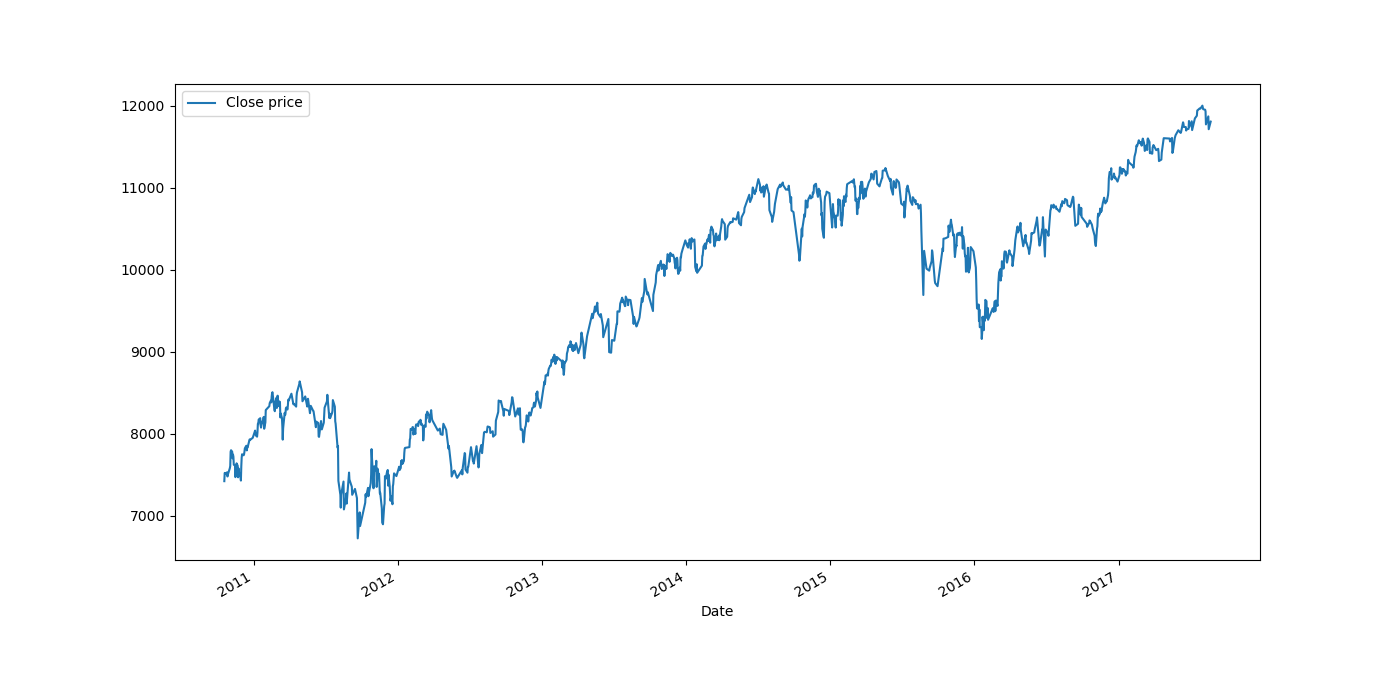
\includegraphics[width=\textwidth]{manuscript/src/figures/Ass4/Ass4_Q2a_raw_signal.png}
    \end{minipage}
    \caption{The raw signal of the dataset.}
    \label{fig:Ass4_Q2a_raw_signal}
\end{figure}

\begin{figure}[H]
    \centering
    \begin{minipage}[b]{1\textwidth}
        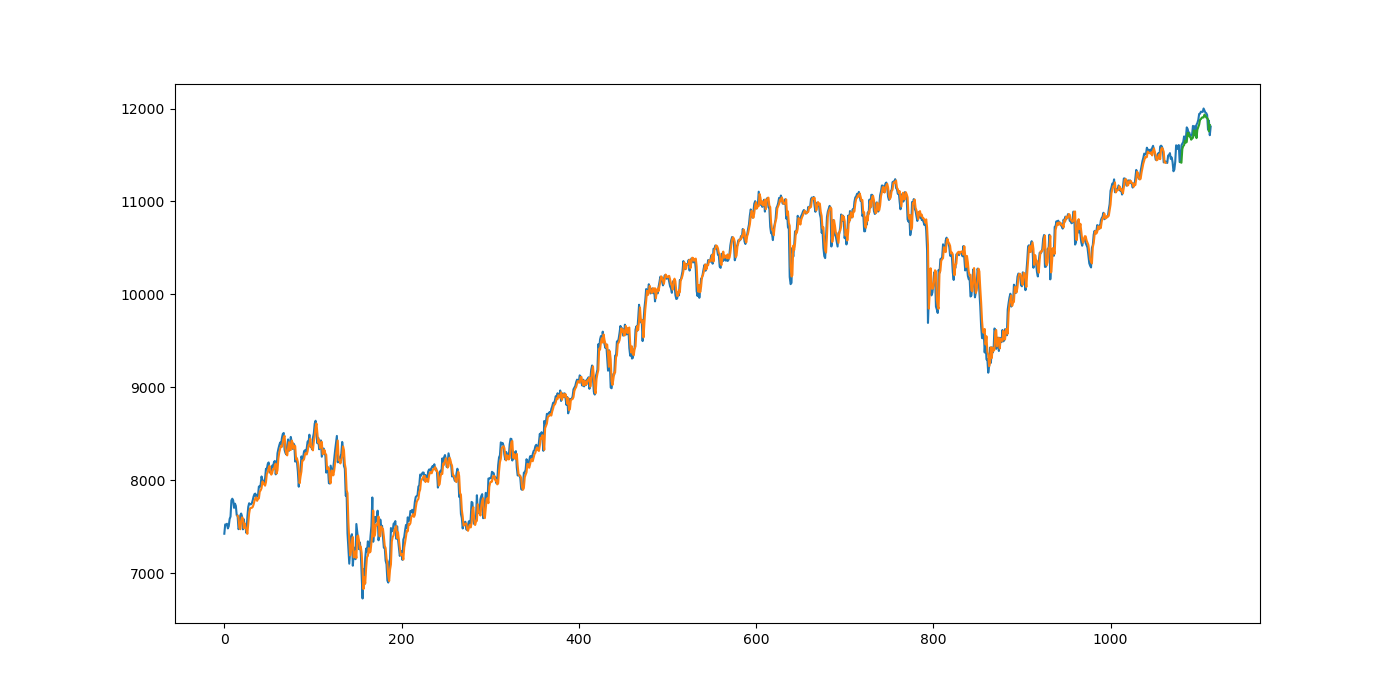
\includegraphics[width=\textwidth]{manuscript/src/figures/Ass4/Ass4_Q2a_forcasted.png}
    \end{minipage}
    \caption{The raw signal of the dataset.}
    \label{fig:Ass4_Q2a_forcasted}
\end{figure}

\begin{figure}[H]
    \centering
    \begin{minipage}[b]{1\textwidth}
        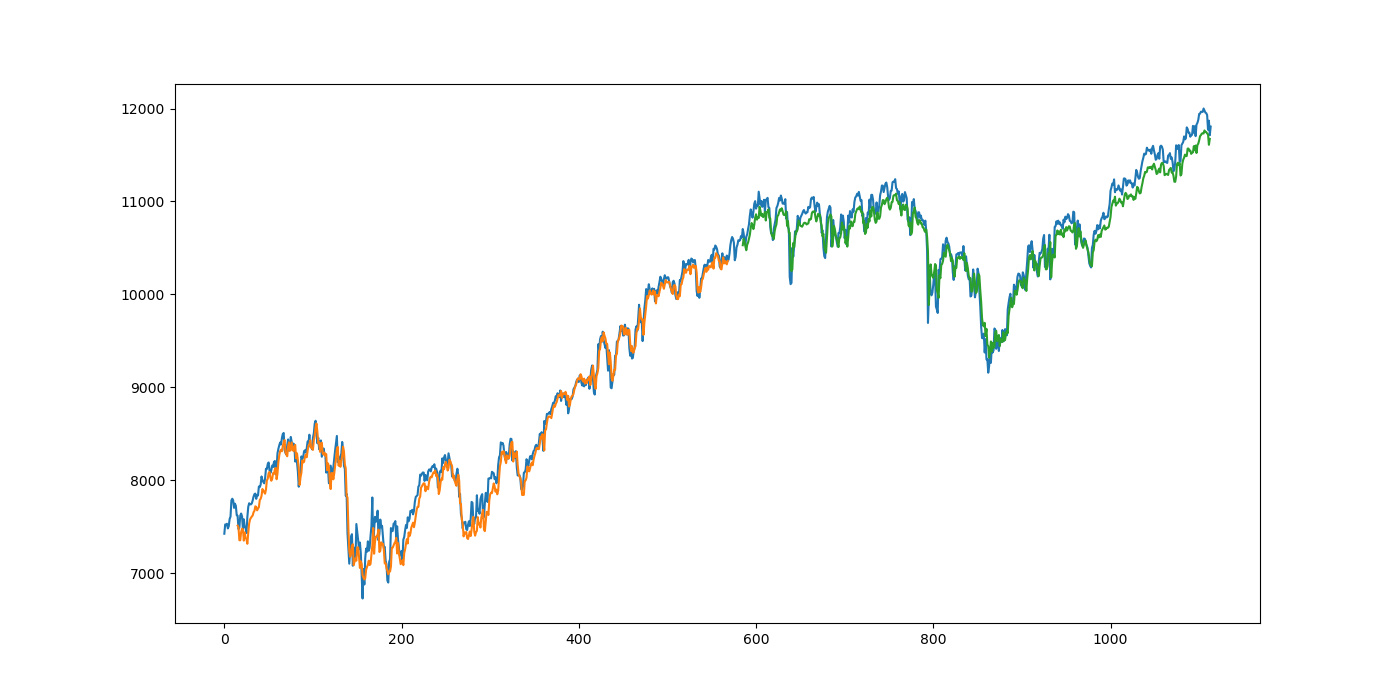
\includegraphics[width=\textwidth]{manuscript/src/figures/Ass4/Ass4_Q2b_forcasted.png}
    \end{minipage}
    \caption{The raw signal of the dataset.}
    \label{fig:Ass4_Q2b_forcasted}
\end{figure}

\begin{figure}[H]
    \centering
    \begin{minipage}[b]{1\textwidth}
        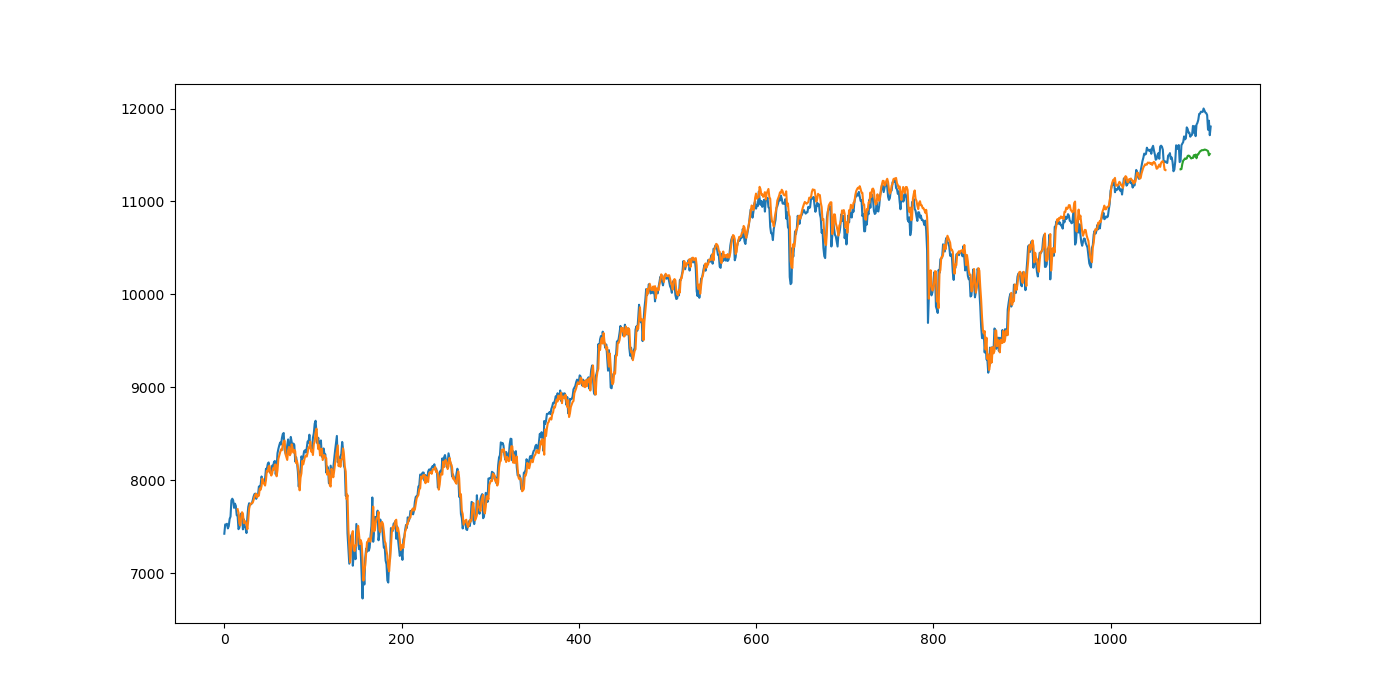
\includegraphics[width=\textwidth]{manuscript/src/figures/Ass4/Ass4_Q2c_forcasted.png}
    \end{minipage}
    \caption{The raw signal of the dataset.}
    \label{fig:Ass4_Q2c_forcasted}
\end{figure}


\begin{figure}[H]
    \centering
    \begin{minipage}[b]{1\textwidth}
        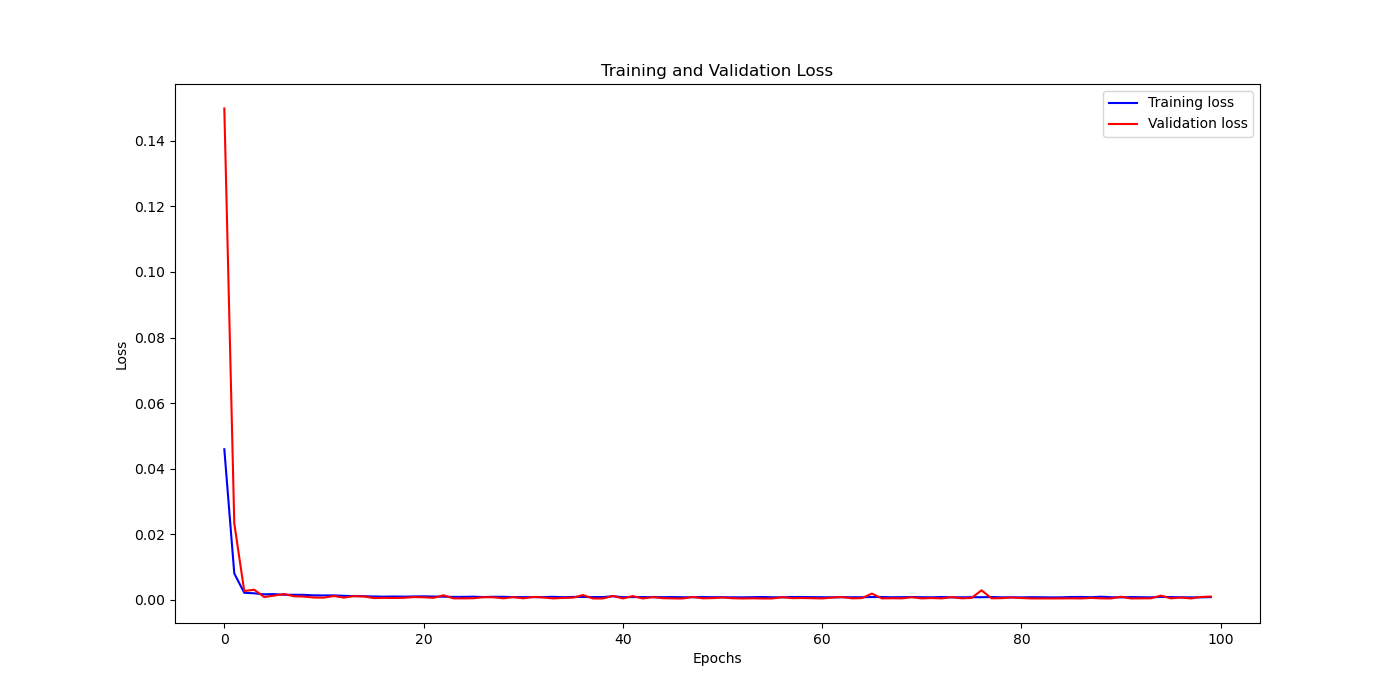
\includegraphics[width=\textwidth]{manuscript/src/figures/Ass4/Ass4_Q2a_Training and Validation Loss.png}
    \end{minipage}
    \caption{The raw signal of the dataset.}
    \label{fig:Ass4_Q2a_Training}
\end{figure}

\begin{figure}[H]
    \centering
    \begin{minipage}[b]{1\textwidth}
        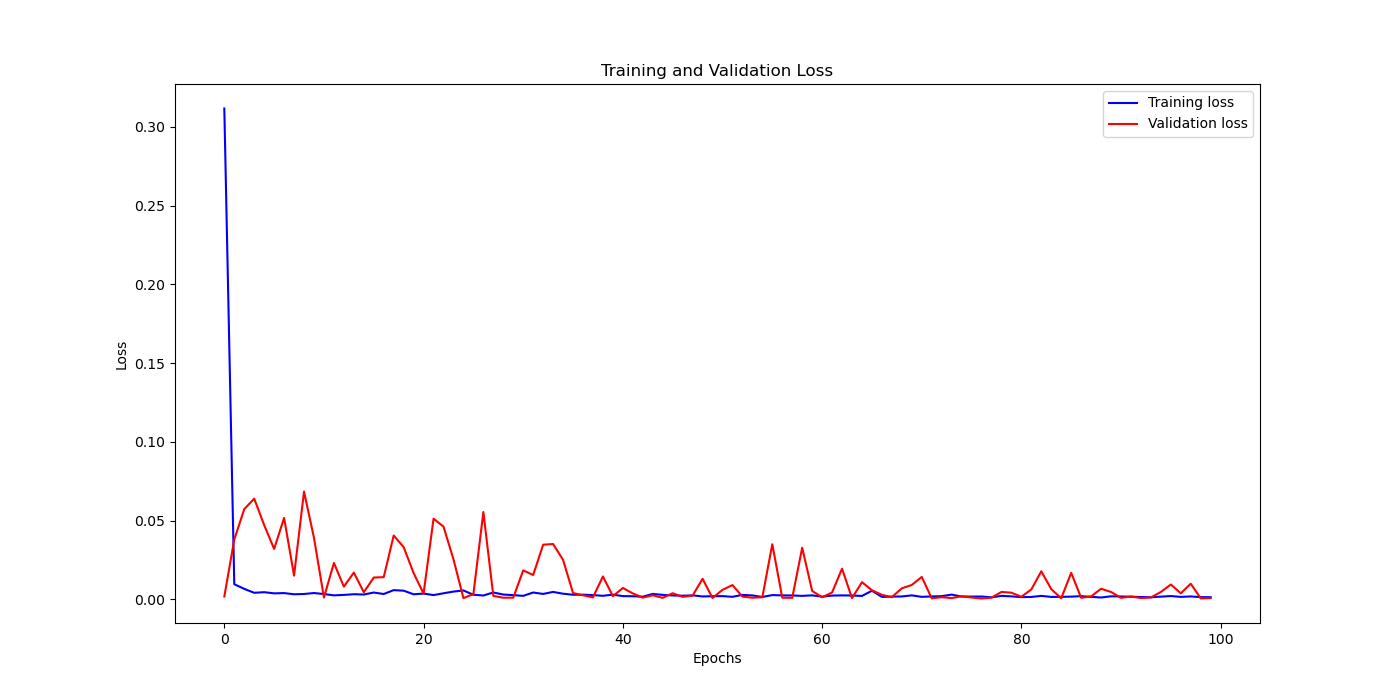
\includegraphics[width=\textwidth]{manuscript/src/figures/Ass4/Ass4_Q2b_Training and Validation Loss.png}
    \end{minipage}
    \caption{The raw signal of the dataset.}
    \label{fig:Ass4_Q2b_Training}
\end{figure}

\begin{figure}[H]
    \centering
    \begin{minipage}[b]{1\textwidth}
        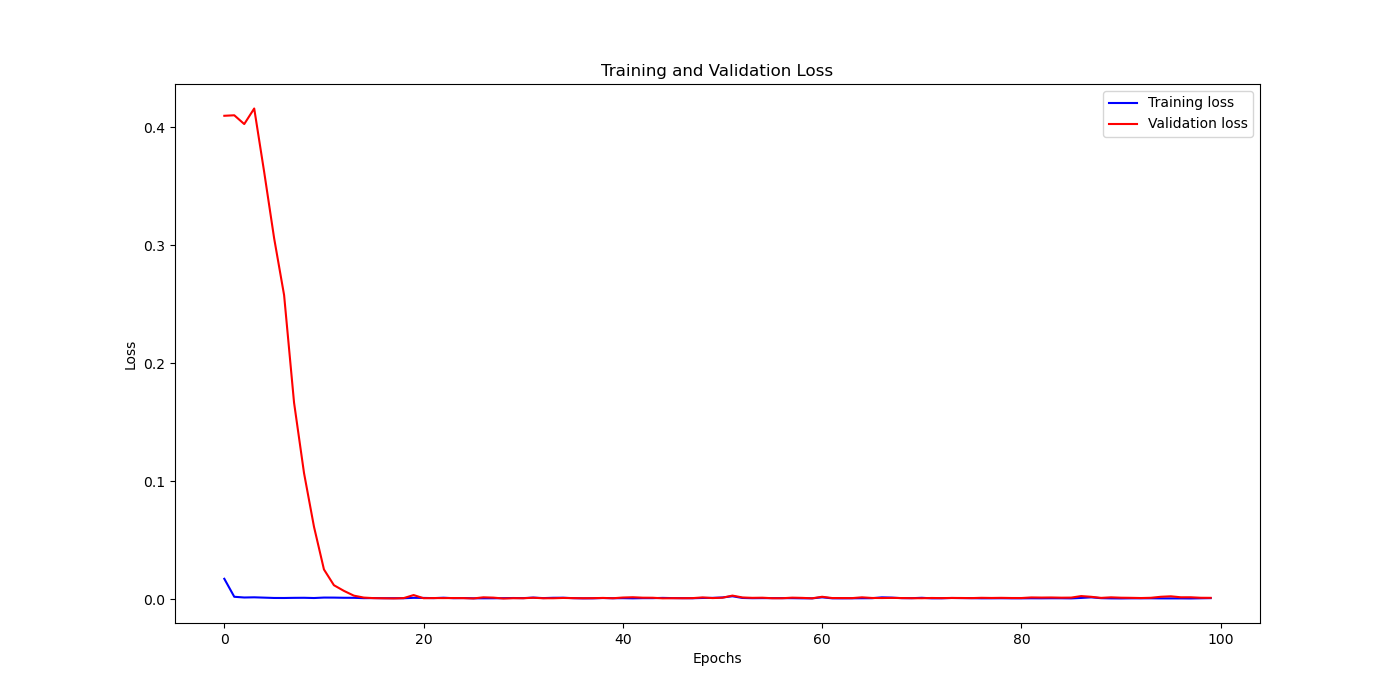
\includegraphics[width=\textwidth]{manuscript/src/figures/Ass4/Ass4_Q2c_Training and Validation Loss.png}
    \end{minipage}
    \caption{The raw signal of the dataset.}
    \label{fig:Ass4_Q2c_Training}
\end{figure}













%%%%%%%%%%%%%%%%%%%%%%%%%%%%%%%%%%%%%%%%%%%%%%%%%%%%%%%%%%%%%%%%%
%%%%%%%%%%%%%%%%%%%%%%%% Question 2 %%%%%%%%%%%%%%%%%%%%%%%%%%%%%
%%%%%%%%%%%%%%%%%%%%%%%%%%%%%%%%%%%%%%%%%%%%%%%%%%%%%%%%%%%%%%%%%
\newpage
\item \textbf{Walk/non-Walk Classification: Train an HMM model to detect the activity ‘Walk’ using users 1-10 for training. Then, use the model to detect ‘walk’ activity patterns in the data from users 11-15. The goal here is to label during which parts of the data the user were walking. You can adjust the selection criteria by varying the likelihood threshold. Compute the system performance/accuracy across different thresholds (hint: explore ROC curves).}

This question is a learning problem. Figure \ref{} indicates the pipeline of my solution. For pre-processing part, we used \emph{re-sampling function} to resize all observations. This could remove the effect of zero padding. After that, 9 varies features were extracted from each each observation signal. for this part, we also considered a window with size of 256 samples and overlap portion of 20 percent.

The output of this section is a matrix with dimension of $3 \times 411 \times 9$ for each activity. 
Then features of each observation (x, y, and z) concatenated to each other to produce a matrix of $411 \times 27$ for each user activity. finally, features were separated based on their activities. the shape of the final array is $15 \times 411 \times 27$; where 15, 411, and 27 indicate number of users, windows, and features respectively.  

In classification part, the array was divided into train and test array. Based on the question, we used users 1 to 10 for training and others for test. Also we set the state variable as loop variable to find the effect of the HMM state in accuracy.

Because we have only one HMM model that was trained for walking activity, the output is the probability. this probability shows whether or not the test features belonged to the this activity. To find the best threshold, we used a \emph{for loop}. The results of this model are illustrated below.  


\begin{table}[H]
\centering
\caption{The results of HMM for different states and thresholds.}
\label{tab:Q2_results}
\begin{tabular}{l}
\toprule
    Test accuracy of 2 states HMM for threshold -10000 : $64.29\%$ \\
    Test accuracy of 2 states HMM for threshold -20000 : 57.14\% \\
    Test accuracy of 2 states HMM for threshold -30000 : 57.14\% \\
    Test accuracy of 2 states HMM for threshold -40000 : 50.00\% \\
    Test accuracy of 2 states HMM for threshold -50000 : 50.00\% \\
    Test accuracy of 2 states HMM for threshold -60000 : 71.43\% \\
    Test accuracy of 2 states HMM for threshold -70000 : \textbf{85.71\%} \\
    Test accuracy of 3 states HMM for threshold -10000 : 64.29\% \\
    Test accuracy of 3 states HMM for threshold -20000 : 50.00\% \\
    Test accuracy of 3 states HMM for threshold -30000 : 50.00\% \\
    Test accuracy of 3 states HMM for threshold -40000 : 42.86\% \\
    Test accuracy of 3 states HMM for threshold -50000 : 50.00\% \\
    Test accuracy of 3 states HMM for threshold -60000 : 50.00\% \\
    Test accuracy of 3 states HMM for threshold -70000 : 57.14\% \\
    Test accuracy of 4 states HMM for threshold -10000 : 57.14\% \\
    Test accuracy of 4 states HMM for threshold -20000 : 57.14\% \\
    Test accuracy of 4 states HMM for threshold -30000 : 50.00\% \\
    Test accuracy of 4 states HMM for threshold -40000 : 57.14\% \\
    Test accuracy of 4 states HMM for threshold -50000 : 50.00\% \\
    Test accuracy of 4 states HMM for threshold -60000 : 50.00\% \\
    Test accuracy of 4 states HMM for threshold -70000 : 57.14\% \\
    Test accuracy of 5 states HMM for threshold -10000 : 64.29\% \\
    Test accuracy of 5 states HMM for threshold -20000 : 64.29\% \\
    Test accuracy of 5 states HMM for threshold -30000 : 64.29\% \\
    Test accuracy of 5 states HMM for threshold -40000 : 64.29\% \\
    Test accuracy of 5 states HMM for threshold -50000 : 57.14\% \\
    Test accuracy of 5 states HMM for threshold -60000 : 57.14\% \\
    Test accuracy of 5 states HMM for threshold -70000 : 57.14\% \\
\bottomrule

\end{tabular}
\end{table}




 

%%%%%%%%%%%%%%%%%%%%%%%%%%%%%%%%%%%%%%%%%%%%%%%%%%%%%%%%%%%%%%%%%
%%%%%%%%%%%%%%%%%%%%%%%% Question 3 %%%%%%%%%%%%%%%%%%%%%%%%%%%%%
%%%%%%%%%%%%%%%%%%%%%%%%%%%%%%%%%%%%%%%%%%%%%%%%%%%%%%%%%%%%%%%%%
\newpage
\item \textbf{Summarize your findings and observations briefly in a final discussion. Submit both the developed code and your document to the Assignment 3 folder on D2L.}
\begin{enumerate}
\item Although re-sampling has some positive effects on features extracting part (deleting zeros padding parts), it could decrease the quality of spectral features. For example, the algorithm could not find any features for this part of the signal because the scale of STFT was changed (see figure \ref{fig:Ass3_Q2_Peak_freq}). Therefore, we need to update our algorithm for finding peaks or extract other features.

\begin{figure}[H]
    \centering
    \begin{minipage}[b]{1\textwidth}
        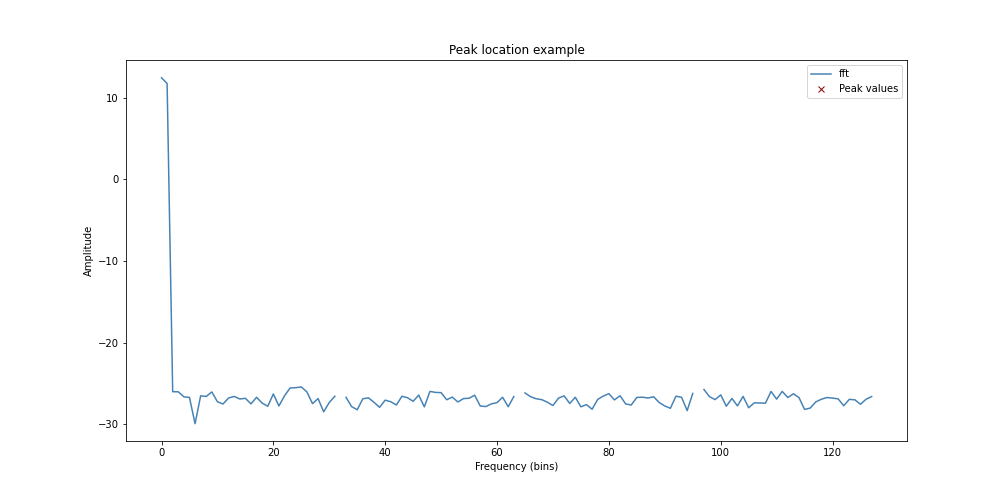
\includegraphics[width=\textwidth]{manuscript/src/figures/Ass3/Ass3_Q2_Peak_freq.png}
    \end{minipage}
    \caption{The magnitude of STFT and its peak values.}
    \label{fig:Ass3_Q2_Peak_freq}
\end{figure}

\item Data normalization had a significant effect on the result of HMM (compare figures \ref{fig:Ass3_Q2_states_user_3} and \ref{fig:Ass3_Q2_states_user_10} with \ref{fig:Ass3_Q2_states_user_3N} and \ref{fig:Ass3_Q2_states_user_10N}, respectively)

\item The decoding result was not good enough for finding different states in raw data. The reason for this result could be either the re-sampling of data or the size of the training set.


\end{enumerate}

%%%%%%%%%%%%%%%%%%%%%%%%%%%%%%%%%%%%%%%%%%%%%%%%%%%%%%%%%%%%%%%%%
%%%%%%%%%%%%%%%%%%%%%%%% Question 4 %%%%%%%%%%%%%%%%%%%%%%%%%%%%%
%%%%%%%%%%%%%%%%%%%%%%%%%%%%%%%%%%%%%%%%%%%%%%%%%%%%%%%%%%%%%%%%%
%\newpage
%\item \textbf{Summarize your findings and observations briefly in a final discussion. Submit both the developed code and your document to the Assignment 1 folder on D2L.}

\textit{All files were uploaded on my GitHub repository \cite{}. The below table, shows the important paths of the project. Beside the codes are available in Appendix }

\begin{table}[H]
\centering
\begin{tabular}{|l|l|}
\hline
\multicolumn{2}{|l|}{The Important Paths:        } \\ \hline
\ \ \ \    ./EE6563/Dataset/Ass1             & Assignment datasets\\ \hline
\ \ \ \    ./EE6563/code/Ass1/sun.py         & Assignment code\\ \hline
\ \ \ \    ./EE6563/code/Ass1/Temp.py        & Assignment code\\ \hline
\ \ \ \    ./EE6563/manuscript/src/figures   & Assignment figures\\ \hline
\ \ \ \    ./EE6563/manuscript/src/tables    & Assignment table\\ \hline
\ \ \ \    ./EE6563/manuscript/src/Ass1.tex  & Assignment document\\ \hline
\end{tabular}
\end{table}












\end{enumerate}



%\newpage
%\section*{REFERENCES}
%\label{sec:sec6}
%\printbibliography[heading=none]

%\bibliography{references}


%\newpage
%\section*{Appendix (codes)}
%\subsection*{The script of sun.py}

%\begin{lstlisting}
%"""https://www.machinelearningplus.com/time-series/time-series-analysis-python/"""
%import warnings

%\end{lstlisting}

\end{document}